%%%%%%%%%%%%%%%%%%%%%%%%%%%%%%%%%%%%%%%%%%
\section{Ottimizzazione del modello di PYTHIA}
Il lavoro principale di questa tesi è stato quello di andare a ottimizzare il parametro \ttbox{norm}.
Originariamente il gruppo di \pythiaa{} aveva calcolato questo parametro scegliendo il valore di $1/\sigma_0$ con energia di centro di massa $\sqrt s = 7$ TeV per il caso dei deuteroni, ossia $1/\sigma_0 = 2.63$ \si{barn^{-1}} (si veda la \autoref{tab:valori_p0_1sigma0}).
Questo dovrebbe spiegare gli andamenti dei grafici in \autoref{fig:A_(anti)deuteron} che non riproducono fedelmente quelli di ALICE.
Quindi si è andati a prendere in considerazione la \autoref{tab:valori_p0_1sigma0} e a cercare di determinare il valore di $1/\sigma_0$ corrispondente a una energia del centro di massa $\sqrt s = 13$ TeV.
Visto che le impostazioni predefinite hanno prodotto una sovrapproduzione, allora vuol dire che $1/\sigma_0$ ha assunto un valore troppo alto per $\sqrt s = 13$ TeV.
Ciò è supportato dal fatto che $1/\sigma_0$ ha un andamento decrescente nella \autoref{tab:valori_p0_1sigma0}.
Quindi l'obiettivo è stato quello di estrapolare questo parametro dalla tabella in questione, facendo attenzione al numero ridotto di punti che si ha a disposizione.

\subsubsection{Fit lineare}
Un primo approccio è stato quello di effettuare un fit lineare ai dati del deuterone per cercare di ottenere un valore preliminare tramite il quale andare a raffinare il parametro.
Tramite questo fit lineare (\autoref{fig:fit_norm}) l'estrapolazione di $1/\sigma_0$ a $\sqrt{s} = 13$ TeV fornisce un valore di $1.7136$ \si{barn^{-1}}, con un valore di $\ttbox{norm} = 183.56$.
\begin{figure}[htb]
    \centering
    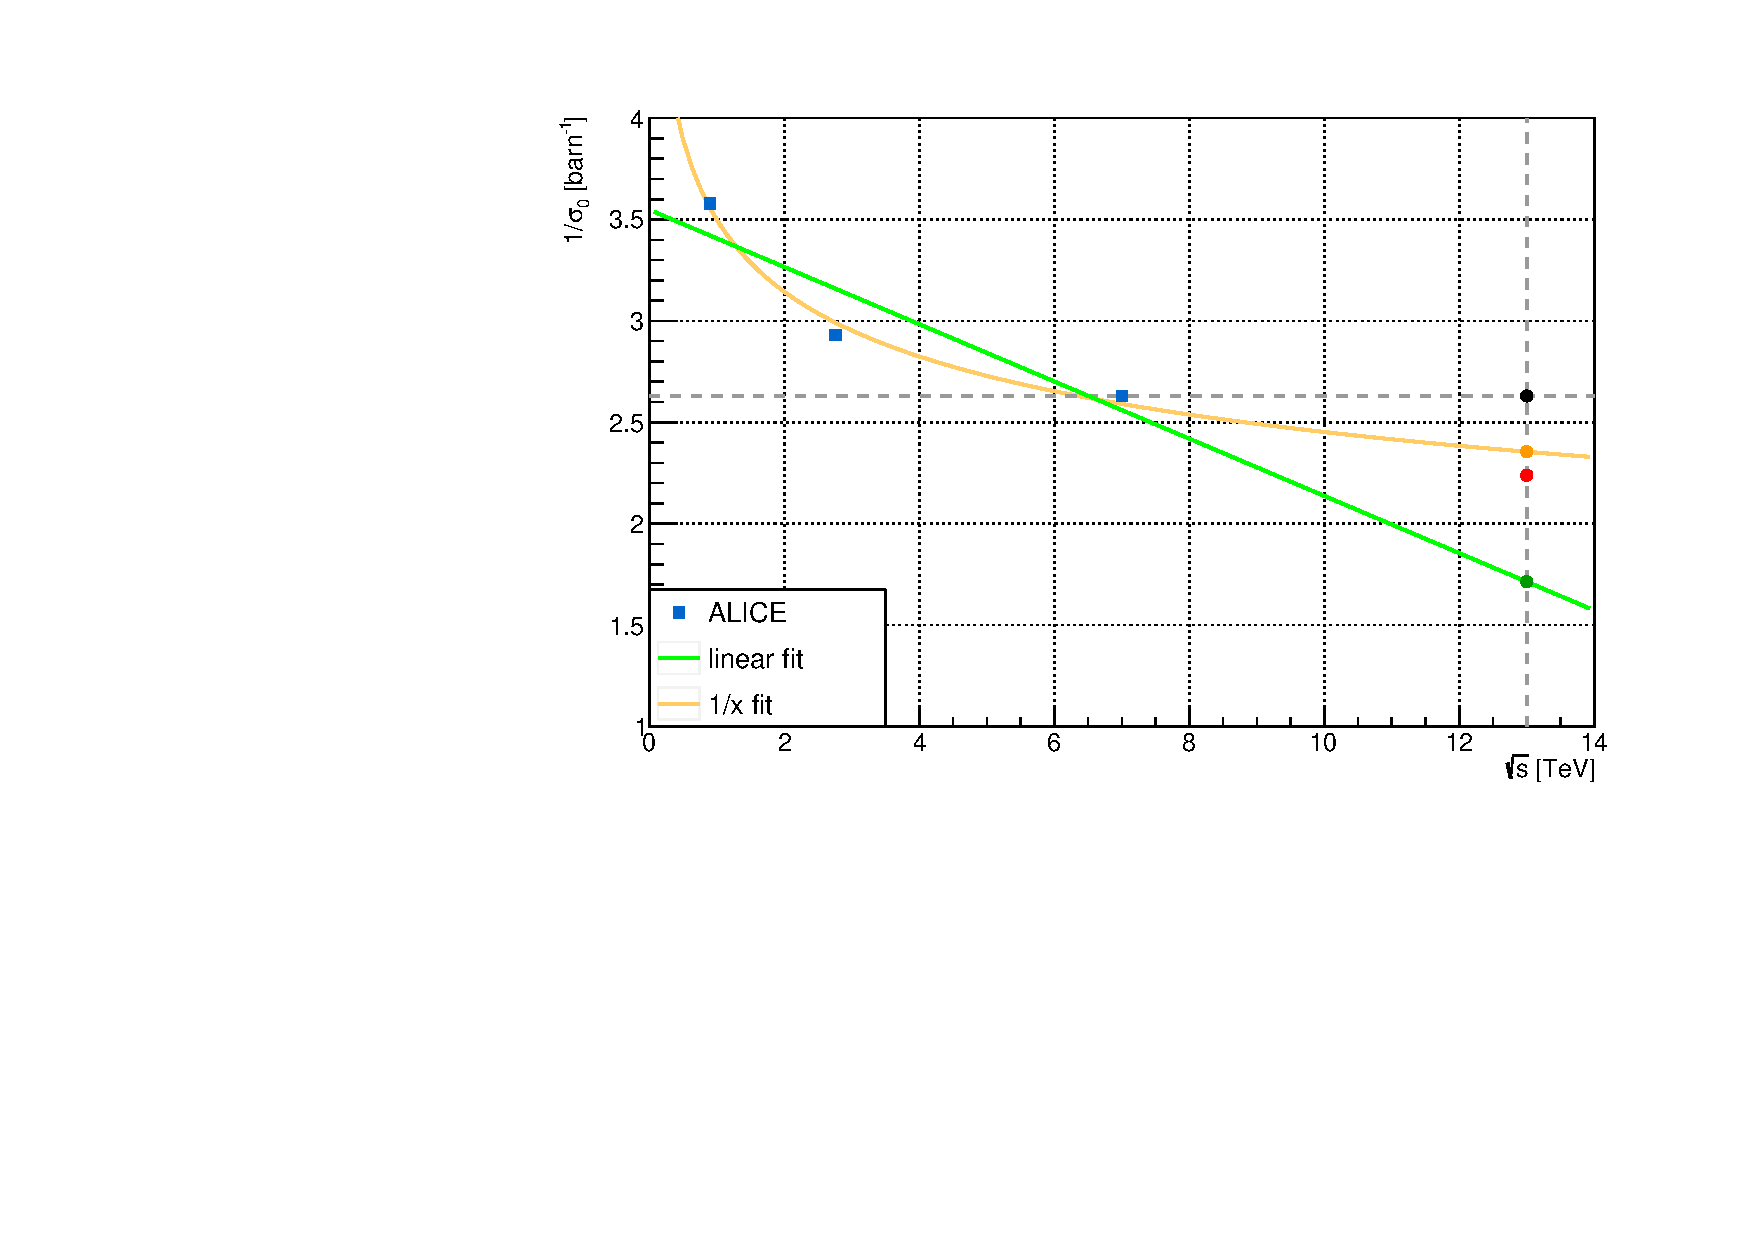
\includegraphics[width=0.9\textwidth]{image/canvas.pdf}
    \caption{Risultati del fit lineare e $1/x$ del parametro $1/\sigma_0$ per i deuteroni. La retta tratteggiata in orizzontale rappresenta $1/\sigma_0 = 2.63$ \si{barn^{-1}}, quella verticale $\sqrt s = 13$ TeV. Su quest'ultima vi sono quattro punti, che in ordine rappresentano (dall'alto verso il basso) il parametro default, del fit $1/x$, ottimizzato e del fit lineare.
    "ALICE" indica i punti derivati da \autoref{tab:valori_p0_1sigma0} nella colonna dei deuteroni.}
    \label{fig:fit_norm}
\end{figure}
Per verificare l'attendibilità di questo valore si è andati a effettuare una simulazione con questo valore di \ttbox{norm} e a confrontare lo spettro di produzione dei (anti)deuteroni con quelli di ALICE.
Le medie pesate derivate dai rapporti tra i dati di \pythiaa{} e di ALICE (in \autoref{fig:B_division}) hanno portato a un valore di $0.789 \pm 0.012$ e $0.746 \pm 0.016$ rispettivamente per i deuteroni e per gli antideuteroni, indicando una sottoproduzione del circa 20-25\%.
Da ciò si può dedurre che il valore $1/\sigma_0$ estrapolato tramite un fit lineare è inferiore rispetto al parametro ideale.
Un fit analogo del parametro $1/\sigma_0$ per gli antideuteroni ha fornito un valore di $1.56872$ \si{barn^{-1}}, corrispondente a $\ttbox{norm} = 200.51$, che tuttavia risulta troppo alto visto il risultato della simulazione con $\ttbox{norm} = 183.56$; tale valore perciò non è stato considerato.

\subsubsection{Fit ${\bf 1/x}$}
Un secondo approccio più realistico è stato quello di tentare di fittare i tre punti con una funzione del tipo
\begin{equation}
    1/\sigma_0\left(\sqrt s\right) = \dfrac{a}{x^b}
\end{equation}
Eseguendo il fit (\autoref{fig:fit_norm}) con questa funzione si è riusciti a ottenere i seguenti valori dei parametri di fit: $a = (3.50 \pm 0.07)$ \si{barn^{-1}} e $b = 0.154 \pm 0.017$.
Così il valore di $1/\sigma_0$ estrapolato a $\sqrt s = 13$ TeV risulta essere di $2.35473$ \si{barn^{-1}}, quindi $\ttbox{norm} = 133.58$, valore accettabile perché compreso tra 119.6 e 183.56.
Eseguendo le simulazioni Monte Carlo con questo parametro si ottiene che gli andamenti degli spettri dei (anti)deuteroni si avvicinano di più ai dati di ALICE rispetto alle simulazioni precedenti.
\begin{figure}[h]
    \centering
    \begin{subfigure}{.49\textwidth}
    \centering
        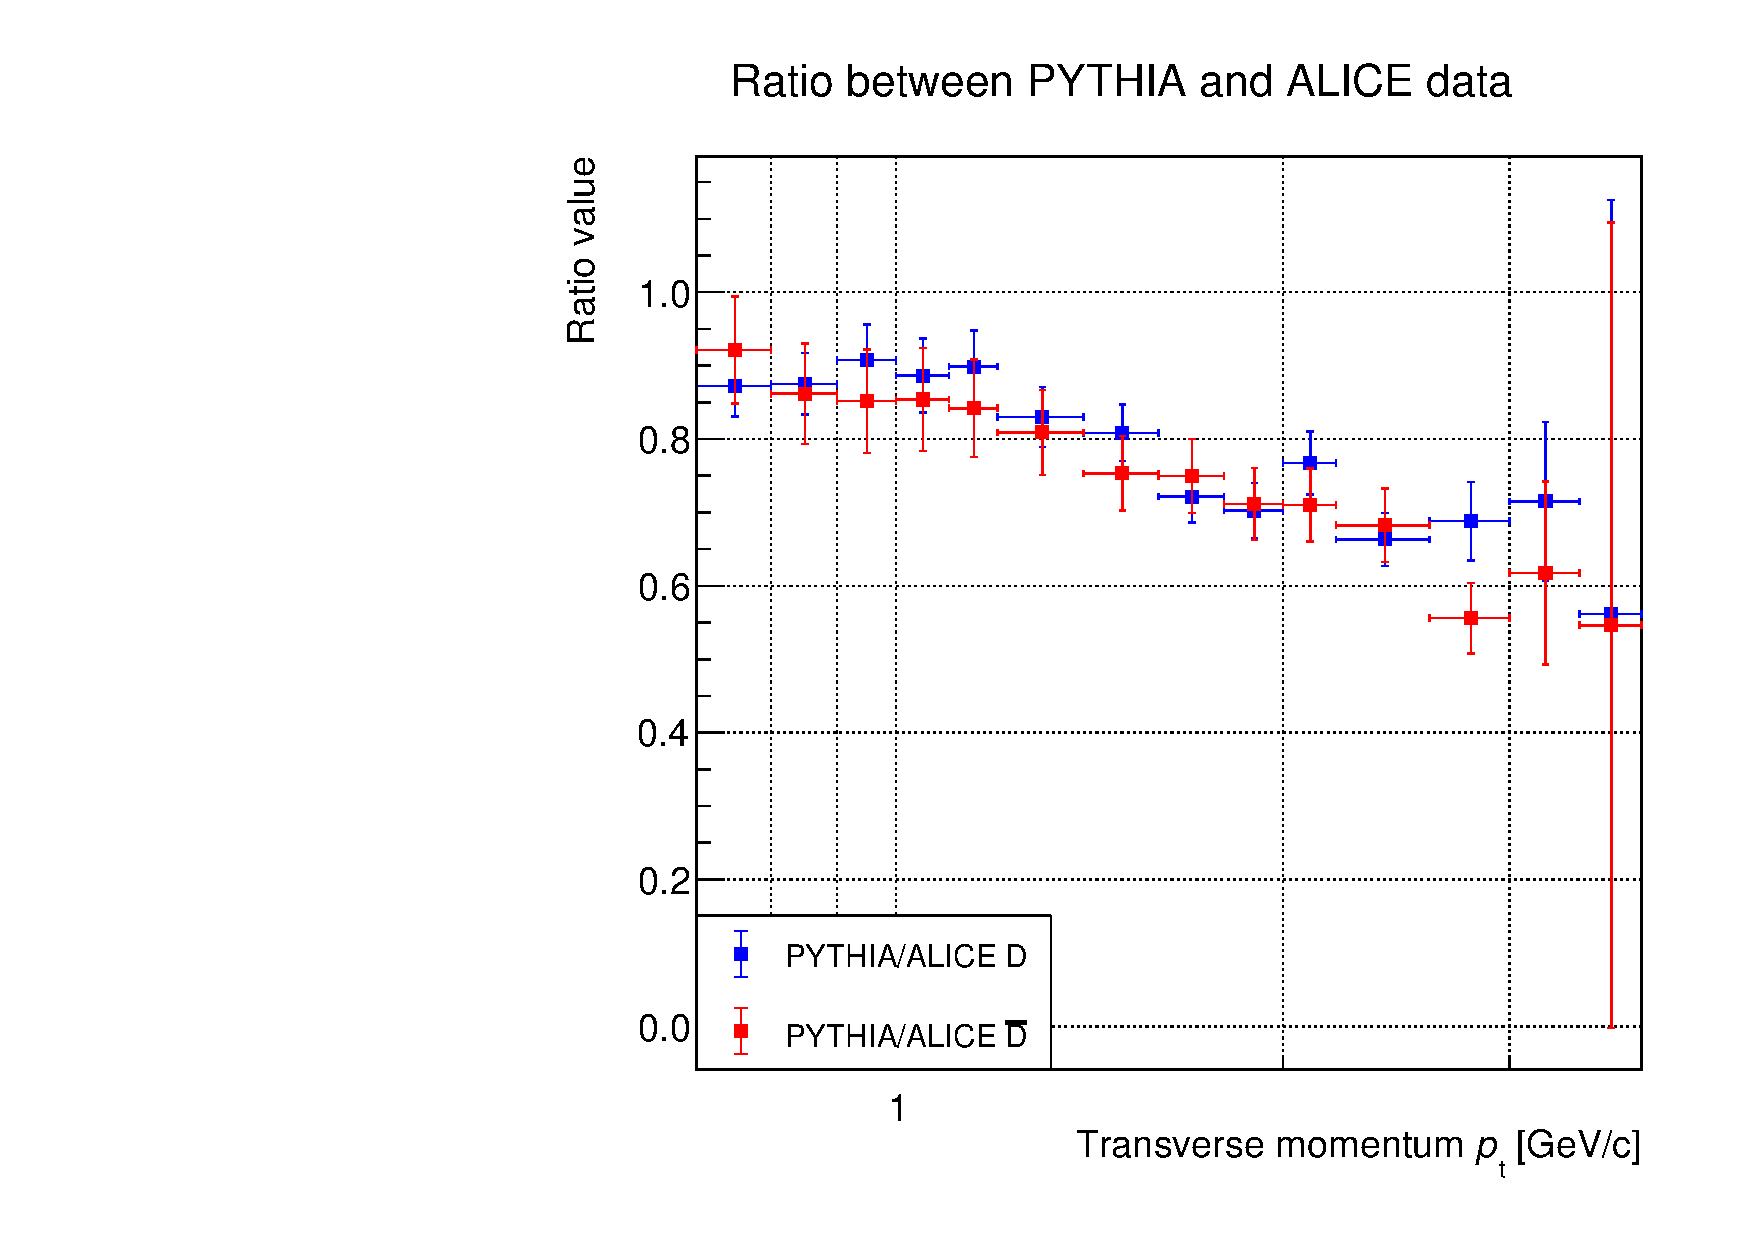
\includegraphics[width=\textwidth]{image/3-risultati/analyse/B/division.pdf}
        \caption{}
        \label{fig:B_division}
    \end{subfigure}
    %\hspace{1cm}
    \begin{subfigure}{.49\textwidth}
        \centering
        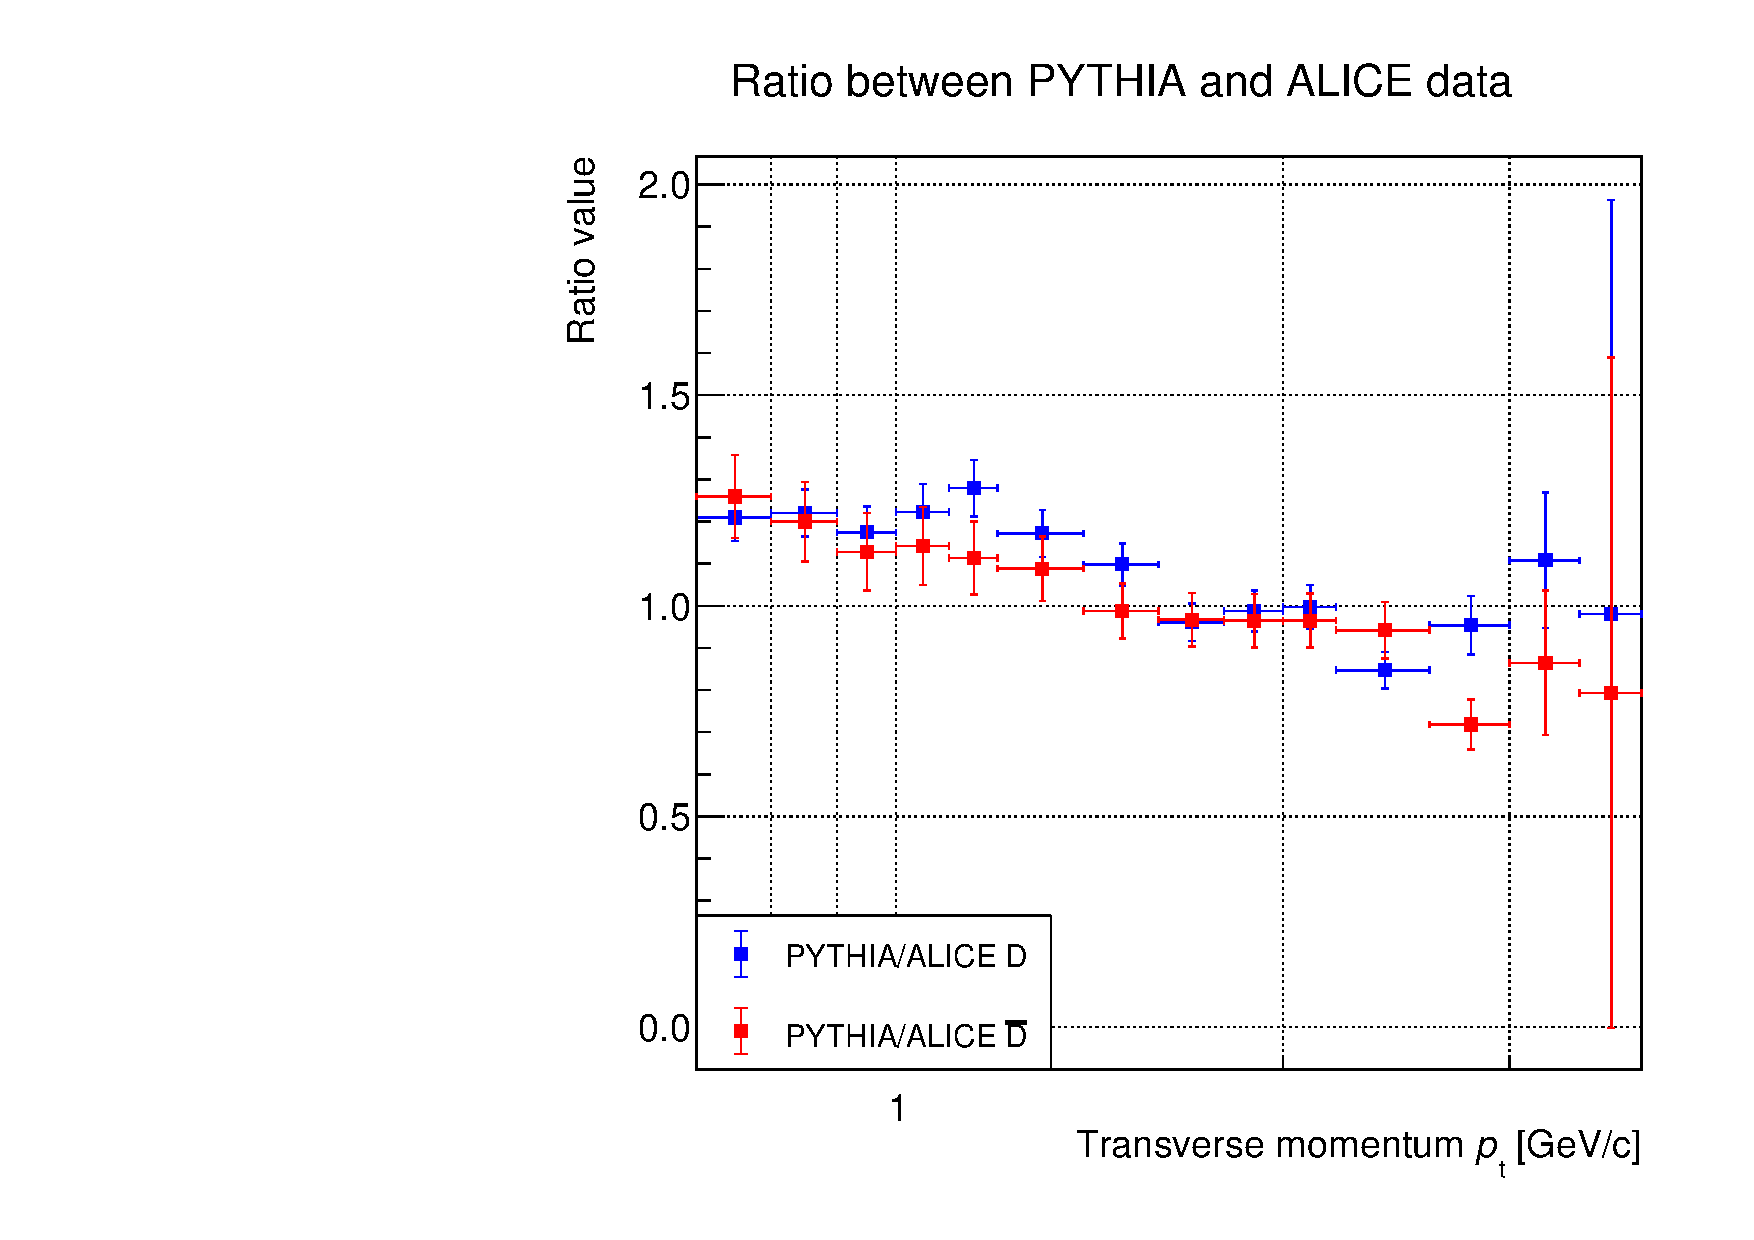
\includegraphics[width=\textwidth]{image/3-risultati/analyse/F/division.pdf}
        \caption{}
        \label{fig:F_division}
    \end{subfigure}
    \caption{Rapporto tra la distribuzione dell'impulso trasverso di $D$ e $\bar D$ con i dati di ALICE \emph{\rmfamily (a)} con \emph{\ttbox{norm}}$=183.56$ e \emph{\rmfamily (b)} con \emph{\ttbox{norm}}$=133.58$.}
    \label{fig:ratio_pp_ON_OFF_BF}
\end{figure}
Questo è supportato dal valore della media pesata del rapporto tra lo spettro dei (anti)deuteroni con i dati di ALICE (\autoref{fig:F_division}) che vale $1.067 \pm 0.015$ e di $0.993 \pm 0.021$ rispettivamente per i deuteroni e per gli antideuteroni. Quindi si nota che il valore di \ttbox{norm} per gli antideuteroni risulta già compatibile entro gli errori con il valore unitario, ma non per i deuteroni.
Questo valore del parametro potrebbe apparire come valore  ottimale, ma ricordando che i valori considerati della \autoref{tab:valori_p0_1sigma0} si riferiscono solamente ai deuteroni, perciò si è proseguiti con l'ottimizzazione del parametro.

\subsubsection{Bisezione}
Per trovare un valore del parametro \ttbox{norm} tale da soddisfare sia la produzione di deuteroni e antideuteroni si è proceduti con un altro metodo alternativo, ispirato al metodo di bisezione.
Per far ciò si correla il parametro \ttbox{norm} con la relativa media pesata.
Andando a considerare i punti del modello predefinito ($\ttbox{norm} = 119.6$, media pesata $= 1.203 \pm 0.017$) e del fit $1/x$ ($\ttbox{norm} = 133.58$, media pesata $= 1.067 \pm 0.03$), si è andati a stimare il valore ottimale del parametro eseguendo empiricamente un fit lineare dei due punti e ricavare il valore del parametro quando la media assume un valore di 1.
Utilizzando questo approccio si è giunti al valore del parametro di $\ttbox{norm} = 140.46721$, leggermente inferiore al parametro derivato dal fit $1/x$.
Eseguendo le simulazioni Monte Carlo ed effettuando il rapporto tra le produzioni di (anti)deuteroni delle simulazioni e di ALICE, otteniamo i valori di media pesata di $1.036 \pm 0.015$ per i deuteroni e $ 0.939 \pm 0.020$ per gli antideuteroni.
Il valore della media pesata per i deuteroni è vicino a 1, ma non è compatibile entro gli errori.
Tuttavia, per semplicità assumiamo questo valore come valore ideale di \ttbox{norm}, e tramite una formula inversa ricaviamo un valore di $1/\sigma_0$ di 2.24 \si{barn^{-1}}.\\

È doveroso notare che, modificando il parametro \ttbox{norm}, quello che si va a fare non è altro che un un semplice riscalaggio agli spettri dei (anti)deuteroni, senza favorire un particolare canali di produzione della \autoref{tab:valori_p0_1sigma0}.
Per cui l'analisi dei canali (e dei loro subcanali) eseguita in \autoref{ch:channels} dovrebbe valere per tutti i valori di \ttbox{norm} (ignorando le regioni in cui si ha meno statistica poiché si avrebbero più fluttuazioni). 